\documentclass[11pt]{article}

\usepackage{lscape,color}
\usepackage{graphicx}
\usepackage[normalem]{ulem}

\topmargin -0.75truein
\oddsidemargin -0.4truein
\textheight 9.25truein
\textwidth 6.7truein
\hbadness=10001
\hfuzz=200pt


\begin{document}
%\input dspace12.tex
%\input pstricks.tex
%\input psfig
\newcommand{\be}{\begin{enumerate}}
\newcommand{\ee}{\end{enumerate}}
\newcommand{\bc}{\begin{center}}
\newcommand{\ec}{\end{center}}
\newcommand{\bi}{\begin{itemize}}
\newcommand{\ei}{\end{itemize}}
\newcommand{\bd}{\begin{description}}
\newcommand{\ed}{\end{description}}
\newcommand{\bt}{\begin{tabbing}}
\newcommand{\et}{\end{tabbing}}
\newcommand{\eg}{{\it e.g.~}}
\newcommand{\ie}{{\it i.e.~}}
\newcommand{\ul}{\underline}
\newcommand{\axaf}{{\em AXAF}}

\def\la{\hbox{\rlap{$<$}\lower0.5ex\hbox{$\sim$}\ }}

\large
%\vspace*{-0.5in}
\centerline {\bf 4.5\_V2.7 TURN ON DEA A}
\vspace{0.25in}

\normalsize
\noindent{\it Last Revised: July 24, 2017}\\
\noindent{\bf Filename: deaa\_on} \\


\noindent {\bf BRIEF FUNCTIONAL DESCRIPTION:} \\
\normalsize
This is an ``atomic'' procedure which simply powers up the DEA side A.
It should be safe to execute under any condition except a spacecraft 
power or thermal emergency.

\vspace{0.25in}
\noindent The sequence of actions for this procedure will be:
\be
\item Verify that DEA B is powered off and disabled (see Constraints/Cautions, below)
\vspace{-0.10in}
\item Verify that DEA A is receiving power from the spacecraft
\vspace{-0.10in}
\item Enable and turn on DEA power supply side A
\vspace{-0.10in}
\item Verify that DEA B is still off
\ee

\vspace{0.15in}
\normalsize
\noindent {\bf ASSUMED INSTRUMENT STATE:}
\normalsize
\be
\item Assumes that the PSMC has power from the spacecraft.
\vspace{-0.10in}
\item Assumes that DEA B is off.
\vspace{-0.10in}
\item Assumes that the DEA was previously powered from side A. If it was instead powered from side B, the board 11 relays must be reset in addition to powering on DEA A.
\ee
\vspace{0.1in}
\normalsize
\noindent {\bf SPECIAL INITIAL CONDITIONS:} \\
\normalsize
%The environment must be clean enough to allow opening of the valve. \\
%Assumes that \axaf\/ ISIM RCTU is powered on and in telemetry format 6. \\

%\vspace{0.25in}
\normalsize
\noindent {\bf OPERATIONAL CONSTRAINTS/CAUTIONS:} \\
\normalsize

In normal operations, only one side of the DEA should be powered on
(a) to prevent conflict for control of the focal plane temperature controller,
(b) to avoid excess current draw from the spacecraft, and (c) to avoid over-heating
within the PSMC.

The DEA power status is normally indicated by the values of the 1DEPSA and
1DEPSB flags, which should not both be 1 simultaneously.
However, if neither side of the DPA is receiving power
({\it i.e.}, if 1DPP0AVO and 1DPP0BVO are simultaneously reading $0.0 \pm 0.5$ V),
the DEA flag values will be unreliable and the DEA voltage
channels (1DEP[0123][AB]VO) should instead be used to determine which
sides of the DEA are powered).

Before sending the command to power on DEA A, the DEA Input Voltage A 1DE28AVO should
be checked to make sure that DEA A is receiving power from the spacecraft.

The DEA input current monitors (1DEIC[AB]CU) are noisy.
To give an indication of what variation may be expected, figures 1 and 2
show the behavior of the A-side DEA current with a ten-sample running
average for two situations in which all video boards were powered down. Note that
when either side of the DEA is unpowered, the corresponding current monitor, 
1DEICACU for side A, or 1DEICBCU for side B, will be unreliable. They will read
16--18~A when unpowered, as of Telemetry Database (TDB) v14. This is expected and
not a problem.

If the DEA powers off unexpectedly during a bakeout, the FP bakeout 
heater will lose power and this heater will NOT be re-enabled when the DEA side A 
power is restored. Additional SW commands are necessary to activate the FP bakeout 
heater. The DH bakeout heater is unaffected by a power loss to the DEA and will 
therefore still be executing a bakeout if power is lost to the DEA.

After successful execution, {\em the FP temperature control will be unregulated,
and DEA interface A/D will be in low-resolution mode.}\\

\vspace{0.15in}
\normalsize
\noindent {\bf REFERENCES:} \\
\normalsize

\normalsize
\noindent {\bf CHANGE HISTORY:} \\
\normalsize

{\bf V1.2}
\begin{itemize}
\item changed filenames from ``turnon\_deaa'' to
``deaa\_on''
\item added text to explain the confusion with the logical verifiers
\end{itemize}

{\bf V1.3}
\begin{itemize}
\item changed HW TLM verifier in step 1.2 to ``1DEN1AVO'' from
``DEN1AVO''
\item changed criticality of +24~V to 1
\item changed TLM FMT to 1,2,4or6
\item added step 1.3 to verify that DEA B is still off
\item added comments to warn that the FP temp will be set to 0~K after the DEA A is powered
\end{itemize}

{\bf V2.0}
\begin{itemize}
\item ACIS Team signed-off version
\item changed HW TLM verifier in step 1.3 to ``1DEN1BVO''
\item edited ``Operational Constraints \& Cautions''
\end{itemize}

{\bf V2.1}
\begin{itemize}
\item Update expected 1DE28AVO range
\item Changed formatting of ``Tlm Fmt'' in table
\item Changed time column from units of seconds to minutes in table
\item Changed text in table column ``Description''
\item Updated expected voltage errors in Step 1.3
\end{itemize}

{\bf V2.2}
\begin{itemize}
\item Update expected 1DEICACU range
\item Add plots showing the behavior of 1DEICACU
\end{itemize}

{\bf V2.3}
\begin{itemize}
\item Added a step to verify DEA-B is off at the beginning of the procedure
\item Moved the text regarding power status issues and expected current behavior from the Functional Description to the Operational Constraints/Cautions section. Also updated the expected FP temperature control.
\end{itemize}

{\bf V2.4}
\begin{itemize}
\item Fixed incorrect 1DEN0AVO and 1DEN1AVO voltages in table
\end{itemize}

{\bf V2.5}
\begin{itemize}
\item Removed input current check for DEA B; added warning to text.
\end{itemize}

{\bf V2.6}
\begin{itemize}
\item Added check of input voltage for DEA A before sending the turn-on command
\item Adjusted values of ``Crit'' column in table. 
\item Note that a bakeout will be interrupted if the DEA powers off, provide details
\end{itemize}

{\bf V2.7}
\begin{itemize}
\item Added a note that this procedure assumes that the DEA was powered from side A and what to do if it wasn't
\end{itemize}

\begin{landscape}
\begin{figure}
\begin{center}
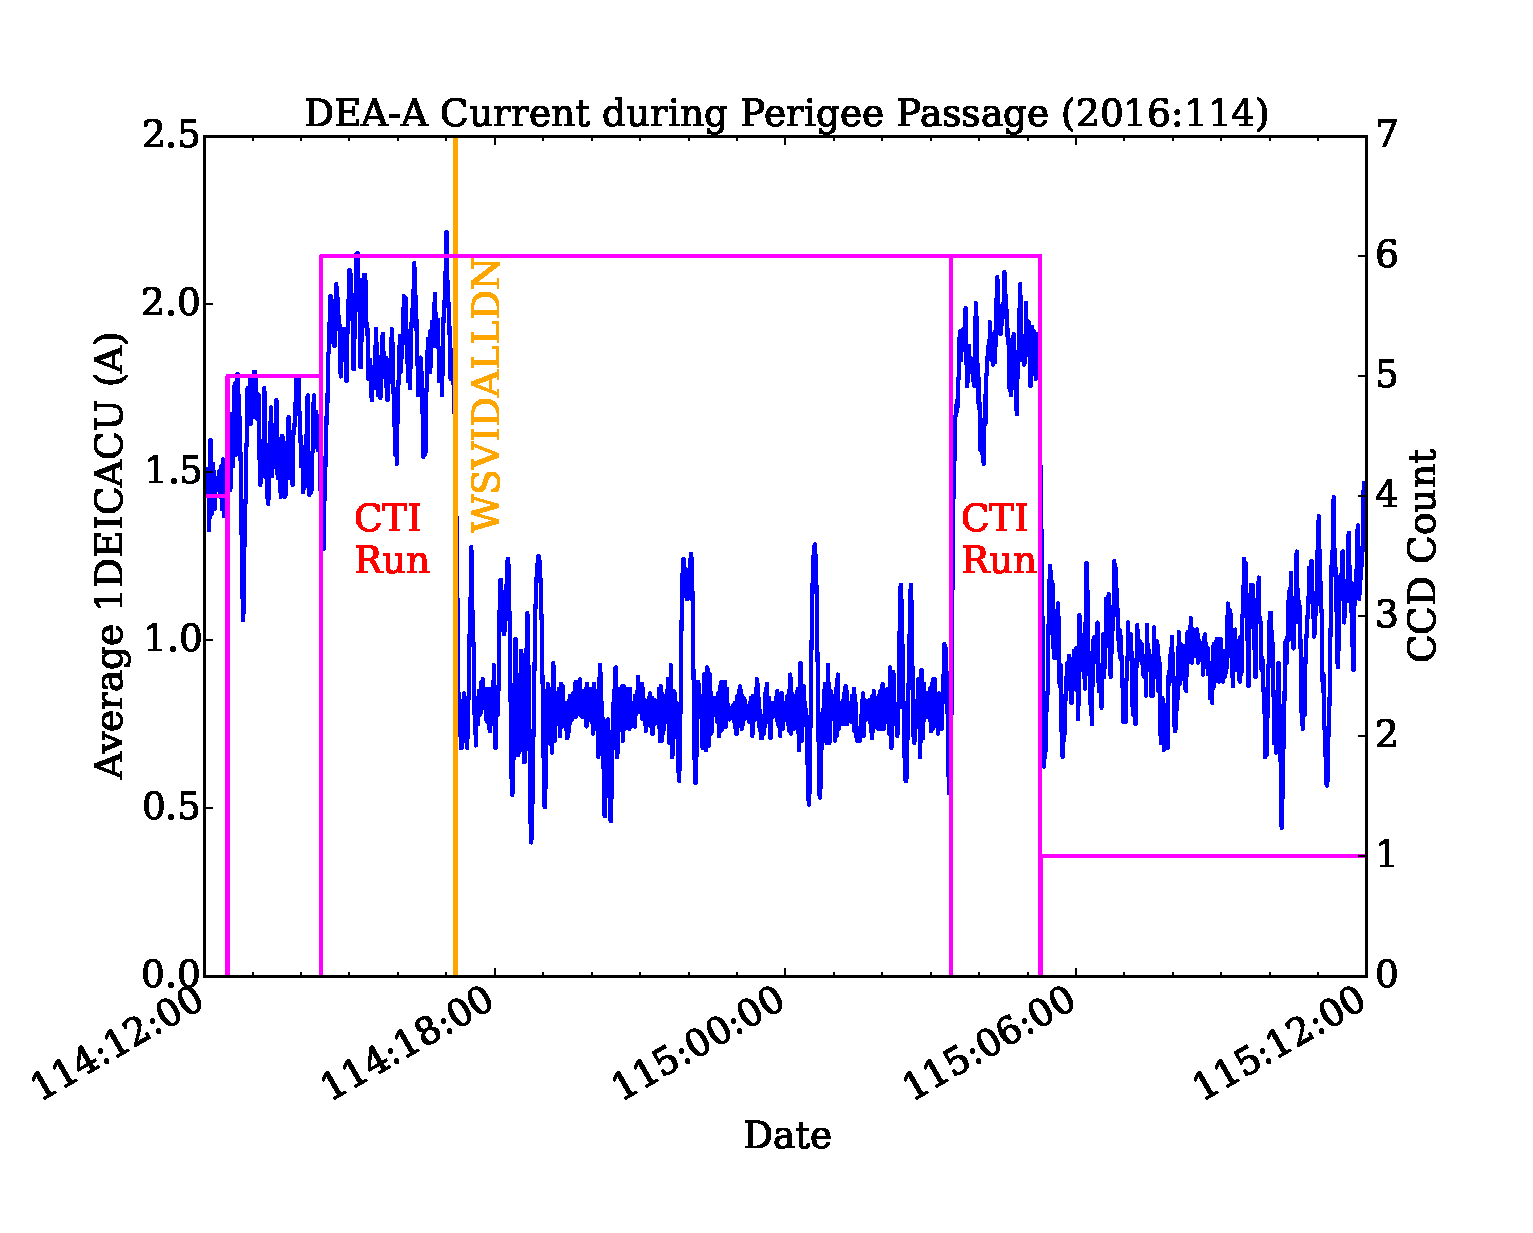
\includegraphics[width=1.2\textwidth]{deaa_on_fig1.eps}
\caption{Ten-sample running average behavior of 1DEICACU during a perigee passage. All video boards
are powered off after the issuing of the WSVIDALLDN command, which is marked by
the orange line in the plot.}
\end{center}
\end{figure}
\end{landscape}

\begin{landscape}
\begin{figure}
\begin{center}
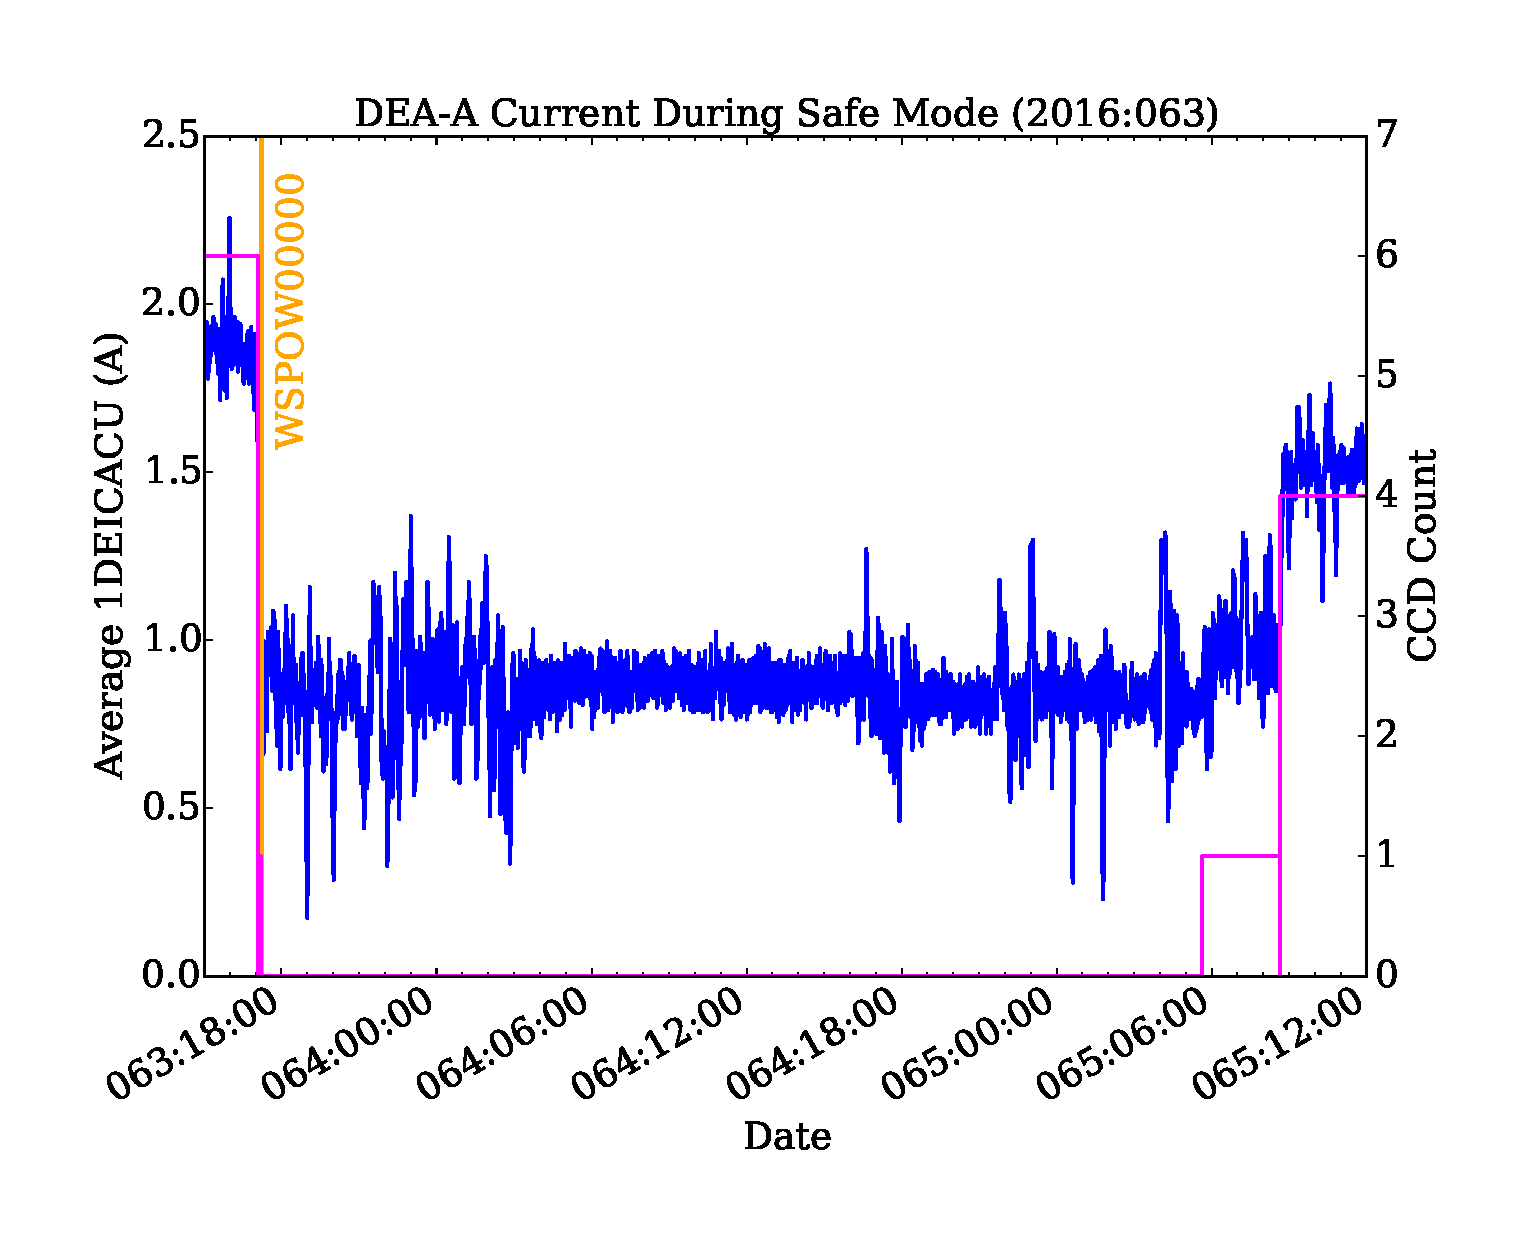
\includegraphics[width=1.2\textwidth]{deaa_on_fig2.eps}
\caption{Ten-sample running average behavior of 1DEICACU during a safe mode. All video boards
are powered off after the issuing of the WSPOW00000 command, which is marked by
the orange line in the plot.}
\end{center}
\end{figure}
\end{landscape}

\newcommand{\tablecaptiontext}{TURN ON DEA A}
\documentclass[11pt]{article}

\usepackage{lscape,color}
\usepackage{graphicx}
\usepackage[normalem]{ulem}

\topmargin -0.75truein
\oddsidemargin -0.4truein
\textheight 9.25truein
\textwidth 6.7truein
\hbadness=10001
\hfuzz=200pt


\begin{document}
%\input dspace12.tex
%\input pstricks.tex
%\input psfig
\newcommand{\be}{\begin{enumerate}}
\newcommand{\ee}{\end{enumerate}}
\newcommand{\bc}{\begin{center}}
\newcommand{\ec}{\end{center}}
\newcommand{\bi}{\begin{itemize}}
\newcommand{\ei}{\end{itemize}}
\newcommand{\bd}{\begin{description}}
\newcommand{\ed}{\end{description}}
\newcommand{\bt}{\begin{tabbing}}
\newcommand{\et}{\end{tabbing}}
\newcommand{\eg}{{\it e.g.~}}
\newcommand{\ie}{{\it i.e.~}}
\newcommand{\ul}{\underline}
\newcommand{\axaf}{{\em AXAF}}

\def\la{\hbox{\rlap{$<$}\lower0.5ex\hbox{$\sim$}\ }}


\large
%\vspace*{-0.5in}
\centerline {\bf 4.5\_V2.6 TURN ON DEA A}
\vspace{0.25in}

\normalsize
\noindent{\it Last Revised: July 11, 2017}\\
\noindent{\bf Filename: deaa\_on} \\


\noindent {\bf BRIEF FUNCTIONAL DESCRIPTION:} \\
\normalsize
This is an ``atomic'' procedure which simply powers up the DEA side A.
It should be safe to execute under any condition except a spacecraft 
power or thermal emergency.

\vspace{0.25in}
\noindent The sequence of actions for this procedure will be:
\be
\item Verify that DEA B is powered off and disabled (see Constraints/Cautions, below)
\vspace{-0.10in}
\item Verify that DEA A is receiving power from the spacecraft
\vspace{-0.10in}
\item Enable and turn on DEA power supply side A
\vspace{-0.10in}
\item Verify that DEA B is still off
\ee

\vspace{0.15in}
\normalsize
\noindent {\bf ASSUMED INSTRUMENT STATE:}
\normalsize
\be
\item Assumes that the PSMC has power from the spacecraft.
\vspace{-0.10in}
\item Assumes that DEA B is off.
\ee
\vspace{0.1in}
\normalsize
\noindent {\bf SPECIAL INITIAL CONDITIONS:} \\
\normalsize
%The environment must be clean enough to allow opening of the valve. \\
%Assumes that \axaf\/ ISIM RCTU is powered on and in telemetry format 6. \\

%\vspace{0.25in}
\normalsize
\noindent {\bf OPERATIONAL CONSTRAINTS/CAUTIONS:} \\
\normalsize

In normal operations, only one side of the DEA should be powered on
(a) to prevent conflict for control of the focal plane temperature controller,
(b) to avoid excess current draw from the spacecraft, and (c) to avoid over-heating
within the PSMC.

The DEA power status is normally indicated by the values of the 1DEPSA and
1DEPSB flags, which should not both be 1 simultaneously.
However, if neither side of the DPA is receiving power
({\it i.e.}, if 1DPP0AVO and 1DPP0BVO are simultaneously reading $0.0 \pm 0.5$ V),
the DEA flag values will be unreliable and the DEA voltage
channels (1DEP[0123][AB]VO) should instead be used to determine which
sides of the DEA are powered).

Before sending the command to power on DEA A, the DEA Input Voltage A 1DE28AVO should
be checked to make sure that DEA A is receiving power from the spacecraft.

The DEA input current monitors (1DEIC[AB]CU) are noisy.
To give an indication of what variation may be expected, figures 1 and 2
show the behavior of the A-side DEA current with a ten-sample running
average for two situations in which all video boards were powered down. Note that
when either side of the DEA is unpowered, the corresponding current monitor, 
1DEICACU for side A, or 1DEICBCU for side B, will be unreliable. They will read
16--18~A when unpowered, as of Telemetry Database (TDB) v14. This is expected and
not a problem.

If the DEA powers off unexpectedly during a bakeout, the FP bakeout 
heater will lose power and this heater will NOT be re-enabled when the DEA side A 
power is restored. Additional SW commands are necessary to activate the FP bakeout 
heater. The DH bakeout heater is unaffected by a power loss to the DEA and will 
therefore still be executing a bakeout if power is lost to the DEA.

After successful execution, {\em the FP temperature control will be unregulated,
and DEA interface A/D will be in low-resolution mode.}\\

\vspace{0.15in}
\normalsize
\noindent {\bf REFERENCES:} \\
\normalsize

\normalsize
\noindent {\bf CHANGE HISTORY:} \\
\normalsize

{\bf V1.2}
\begin{itemize}
\item changed filenames from ``turnon\_deaa'' to
``deaa\_on''
\item added text to explain the confusion with the logical verifiers
\end{itemize}

{\bf V1.3}
\begin{itemize}
\item changed HW TLM verifier in step 1.2 to ``1DEN1AVO'' from
``DEN1AVO''
\item changed criticality of +24~V to 1
\item changed TLM FMT to 1,2,4or6
\item added step 1.3 to verify that DEA B is still off
\item added comments to warn that the FP temp will be set to 0~K after the DEA A is powered
\end{itemize}

{\bf V2.0}
\begin{itemize}
\item ACIS Team signed-off version
\item changed HW TLM verifier in step 1.3 to ``1DEN1BVO''
\item edited ``Operational Constraints \& Cautions''
\end{itemize}

{\bf V2.1}
\begin{itemize}
\item Update expected 1DE28AVO range
\item Changed formatting of ``Tlm Fmt'' in table
\item Changed time column from units of seconds to minutes in table
\item Changed text in table column ``Description''
\item Updated expected voltage errors in Step 1.3
\end{itemize}

{\bf V2.2}
\begin{itemize}
\item Update expected 1DEICACU range
\item Add plots showing the behavior of 1DEICACU
\end{itemize}

{\bf V2.3}
\begin{itemize}
\item Added a step to verify DEA-B is off at the beginning of the procedure
\item Moved the text regarding power status issues and expected current behavior from the Functional Description to the Operational Constraints/Cautions section. Also updated the expected FP temperature control.
\end{itemize}

{\bf V2.4}
\begin{itemize}
\item Fixed incorrect 1DEN0AVO and 1DEN1AVO voltages in table
\end{itemize}

{\bf V2.5}
\begin{itemize}
\item Removed input current check for DEA B; added warning to text.
\end{itemize}

{\bf V2.6}
\begin{itemize}
\item Added check of input voltage for DEA A before sending the turn-on command
\item Adjusted values of ``Crit'' column in table. 
\item Note that a bakeout will be interrupted if the DEA powers off, provide details
\end{itemize}

\begin{landscape}
\begin{figure}
\begin{center}
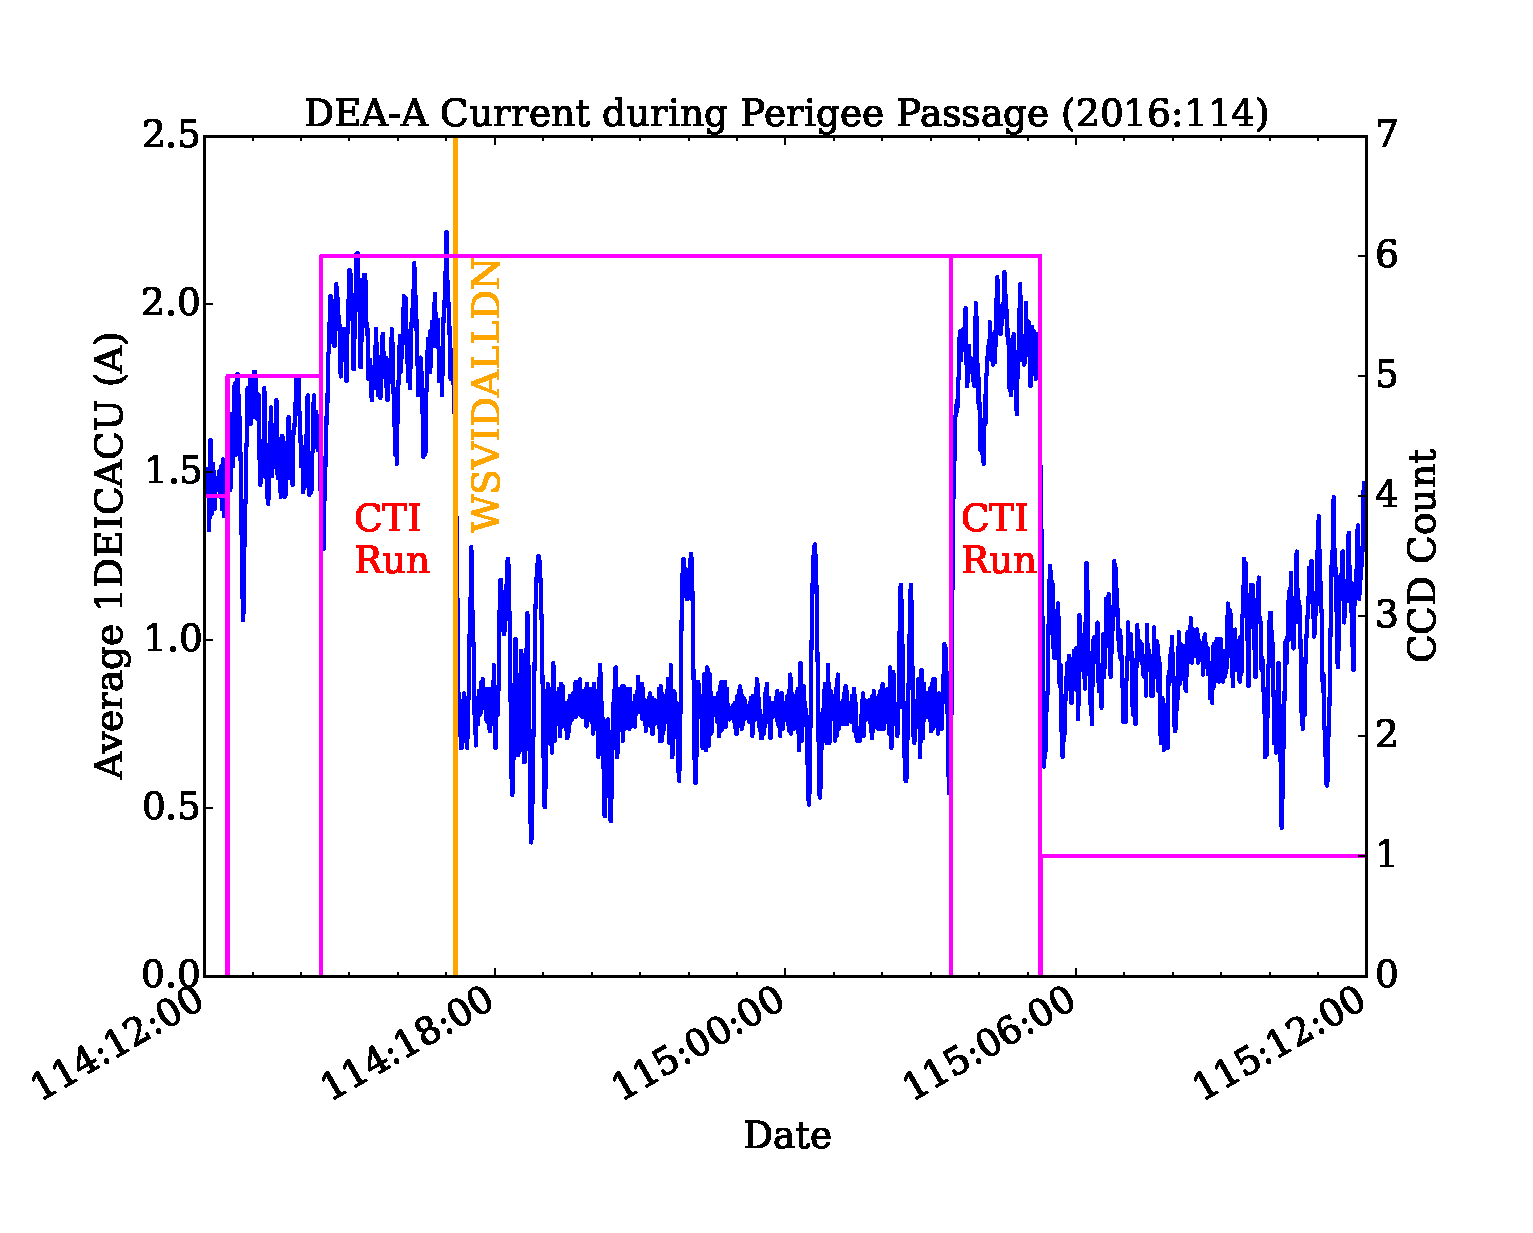
\includegraphics[width=1.2\textwidth]{deaa_on_fig1.eps}
\caption{Ten-sample running average behavior of 1DEICACU during a perigee passage. All video boards
are powered off after the issuing of the WSVIDALLDN command, which is marked by
the orange line in the plot.}
\end{center}
\end{figure}
\end{landscape}

\begin{landscape}
\begin{figure}
\begin{center}
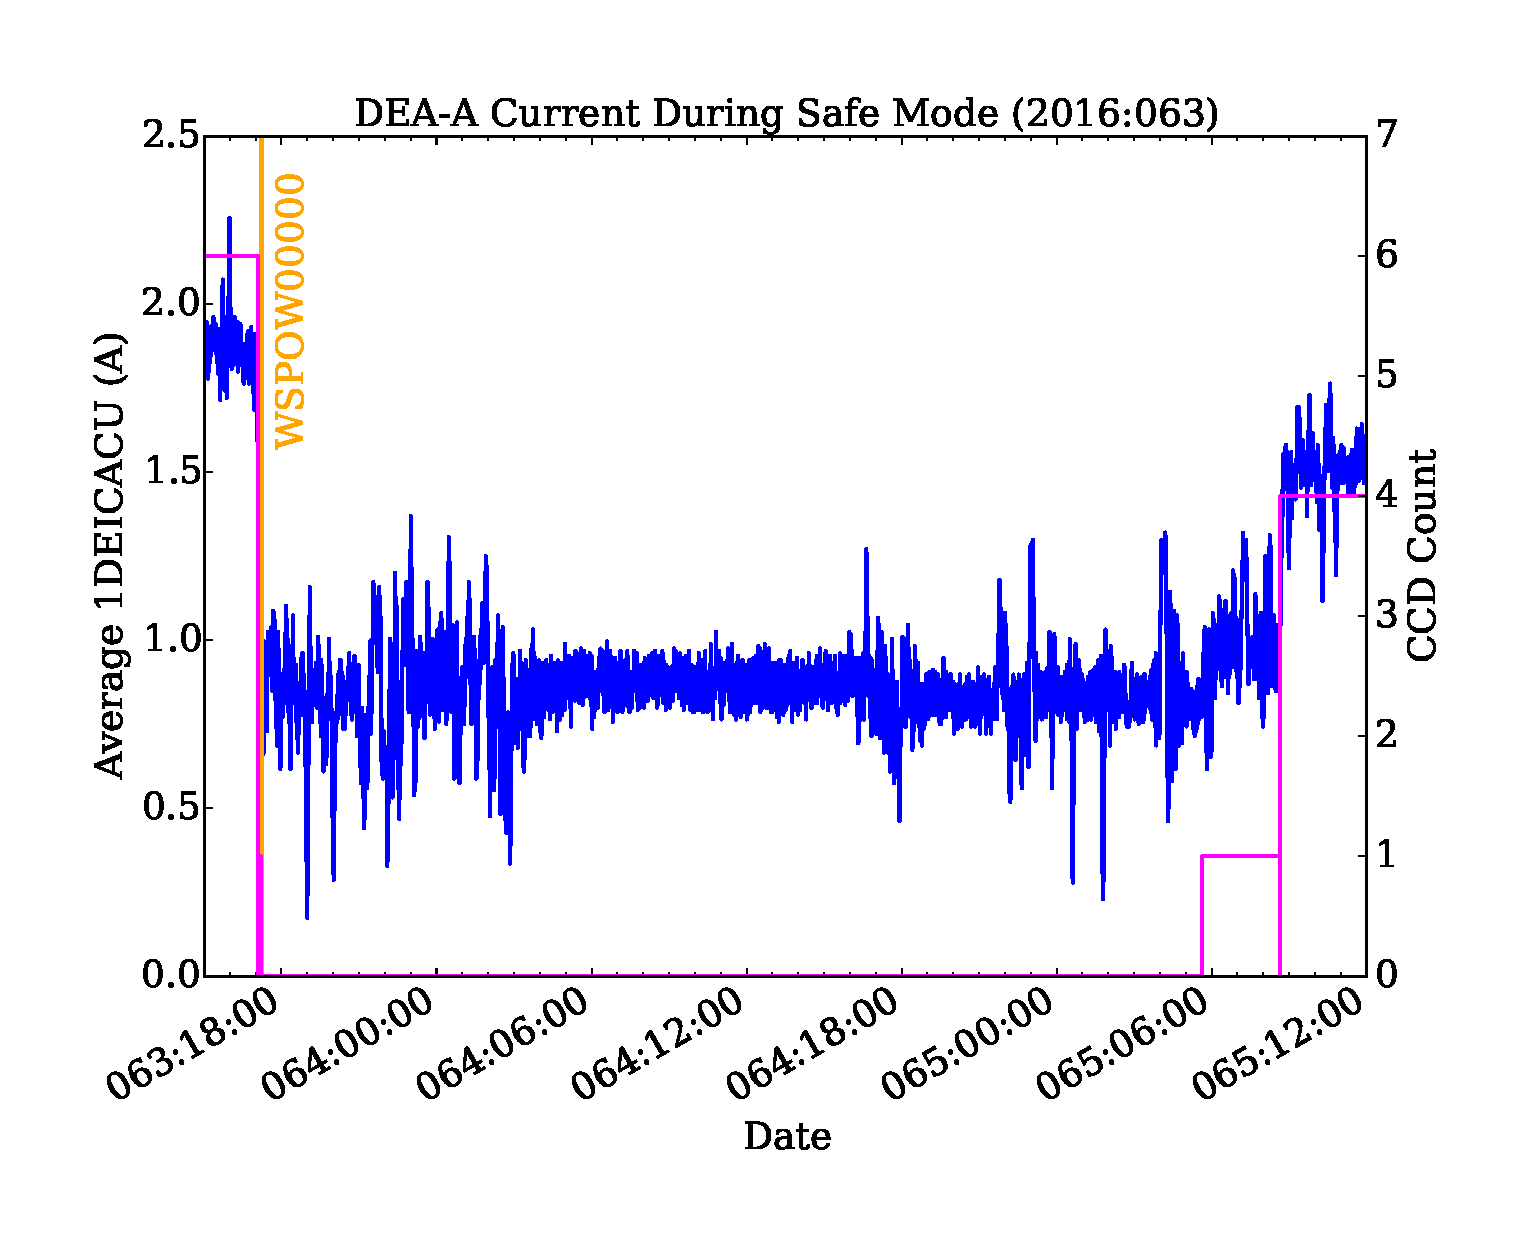
\includegraphics[width=1.2\textwidth]{deaa_on_fig2.eps}
\caption{Ten-sample running average behavior of 1DEICACU during a safe mode. All video boards
are powered off after the issuing of the WSPOW00000 command, which is marked by
the orange line in the plot.}
\end{center}
\end{figure}
\end{landscape}

\newcommand{\tablecaptiontext}{TURN ON DEA A}
\documentclass[11pt]{article}

\usepackage{lscape,color}
\usepackage{graphicx}
\usepackage[normalem]{ulem}

\topmargin -0.75truein
\oddsidemargin -0.4truein
\textheight 9.25truein
\textwidth 6.7truein
\hbadness=10001
\hfuzz=200pt


\begin{document}
%\input dspace12.tex
%\input pstricks.tex
%\input psfig
\newcommand{\be}{\begin{enumerate}}
\newcommand{\ee}{\end{enumerate}}
\newcommand{\bc}{\begin{center}}
\newcommand{\ec}{\end{center}}
\newcommand{\bi}{\begin{itemize}}
\newcommand{\ei}{\end{itemize}}
\newcommand{\bd}{\begin{description}}
\newcommand{\ed}{\end{description}}
\newcommand{\bt}{\begin{tabbing}}
\newcommand{\et}{\end{tabbing}}
\newcommand{\eg}{{\it e.g.~}}
\newcommand{\ie}{{\it i.e.~}}
\newcommand{\ul}{\underline}
\newcommand{\axaf}{{\em AXAF}}

\def\la{\hbox{\rlap{$<$}\lower0.5ex\hbox{$\sim$}\ }}


\large
%\vspace*{-0.5in}
\centerline {\bf 4.5\_V2.6 TURN ON DEA A}
\vspace{0.25in}

\normalsize
\noindent{\it Last Revised: July 11, 2017}\\
\noindent{\bf Filename: deaa\_on} \\


\noindent {\bf BRIEF FUNCTIONAL DESCRIPTION:} \\
\normalsize
This is an ``atomic'' procedure which simply powers up the DEA side A.
It should be safe to execute under any condition except a spacecraft 
power or thermal emergency.

\vspace{0.25in}
\noindent The sequence of actions for this procedure will be:
\be
\item Verify that DEA B is powered off and disabled (see Constraints/Cautions, below)
\vspace{-0.10in}
\item Verify that DEA A is receiving power from the spacecraft
\vspace{-0.10in}
\item Enable and turn on DEA power supply side A
\vspace{-0.10in}
\item Verify that DEA B is still off
\ee

\vspace{0.15in}
\normalsize
\noindent {\bf ASSUMED INSTRUMENT STATE:}
\normalsize
\be
\item Assumes that the PSMC has power from the spacecraft.
\vspace{-0.10in}
\item Assumes that DEA B is off.
\ee
\vspace{0.1in}
\normalsize
\noindent {\bf SPECIAL INITIAL CONDITIONS:} \\
\normalsize
%The environment must be clean enough to allow opening of the valve. \\
%Assumes that \axaf\/ ISIM RCTU is powered on and in telemetry format 6. \\

%\vspace{0.25in}
\normalsize
\noindent {\bf OPERATIONAL CONSTRAINTS/CAUTIONS:} \\
\normalsize

In normal operations, only one side of the DEA should be powered on
(a) to prevent conflict for control of the focal plane temperature controller,
(b) to avoid excess current draw from the spacecraft, and (c) to avoid over-heating
within the PSMC.

The DEA power status is normally indicated by the values of the 1DEPSA and
1DEPSB flags, which should not both be 1 simultaneously.
However, if neither side of the DPA is receiving power
({\it i.e.}, if 1DPP0AVO and 1DPP0BVO are simultaneously reading $0.0 \pm 0.5$ V),
the DEA flag values will be unreliable and the DEA voltage
channels (1DEP[0123][AB]VO) should instead be used to determine which
sides of the DEA are powered).

Before sending the command to power on DEA A, the DEA Input Voltage A 1DE28AVO should
be checked to make sure that DEA A is receiving power from the spacecraft.

The DEA input current monitors (1DEIC[AB]CU) are noisy.
To give an indication of what variation may be expected, figures 1 and 2
show the behavior of the A-side DEA current with a ten-sample running
average for two situations in which all video boards were powered down. Note that
when either side of the DEA is unpowered, the corresponding current monitor, 
1DEICACU for side A, or 1DEICBCU for side B, will be unreliable. They will read
16--18~A when unpowered, as of Telemetry Database (TDB) v14. This is expected and
not a problem.

If the DEA powers off unexpectedly during a bakeout, the FP bakeout 
heater will lose power and this heater will NOT be re-enabled when the DEA side A 
power is restored. Additional SW commands are necessary to activate the FP bakeout 
heater. The DH bakeout heater is unaffected by a power loss to the DEA and will 
therefore still be executing a bakeout if power is lost to the DEA.

After successful execution, {\em the FP temperature control will be unregulated,
and DEA interface A/D will be in low-resolution mode.}\\

\vspace{0.15in}
\normalsize
\noindent {\bf REFERENCES:} \\
\normalsize

\normalsize
\noindent {\bf CHANGE HISTORY:} \\
\normalsize

{\bf V1.2}
\begin{itemize}
\item changed filenames from ``turnon\_deaa'' to
``deaa\_on''
\item added text to explain the confusion with the logical verifiers
\end{itemize}

{\bf V1.3}
\begin{itemize}
\item changed HW TLM verifier in step 1.2 to ``1DEN1AVO'' from
``DEN1AVO''
\item changed criticality of +24~V to 1
\item changed TLM FMT to 1,2,4or6
\item added step 1.3 to verify that DEA B is still off
\item added comments to warn that the FP temp will be set to 0~K after the DEA A is powered
\end{itemize}

{\bf V2.0}
\begin{itemize}
\item ACIS Team signed-off version
\item changed HW TLM verifier in step 1.3 to ``1DEN1BVO''
\item edited ``Operational Constraints \& Cautions''
\end{itemize}

{\bf V2.1}
\begin{itemize}
\item Update expected 1DE28AVO range
\item Changed formatting of ``Tlm Fmt'' in table
\item Changed time column from units of seconds to minutes in table
\item Changed text in table column ``Description''
\item Updated expected voltage errors in Step 1.3
\end{itemize}

{\bf V2.2}
\begin{itemize}
\item Update expected 1DEICACU range
\item Add plots showing the behavior of 1DEICACU
\end{itemize}

{\bf V2.3}
\begin{itemize}
\item Added a step to verify DEA-B is off at the beginning of the procedure
\item Moved the text regarding power status issues and expected current behavior from the Functional Description to the Operational Constraints/Cautions section. Also updated the expected FP temperature control.
\end{itemize}

{\bf V2.4}
\begin{itemize}
\item Fixed incorrect 1DEN0AVO and 1DEN1AVO voltages in table
\end{itemize}

{\bf V2.5}
\begin{itemize}
\item Removed input current check for DEA B; added warning to text.
\end{itemize}

{\bf V2.6}
\begin{itemize}
\item Added check of input voltage for DEA A before sending the turn-on command
\item Adjusted values of ``Crit'' column in table. 
\item Note that a bakeout will be interrupted if the DEA powers off, provide details
\end{itemize}

\begin{landscape}
\begin{figure}
\begin{center}
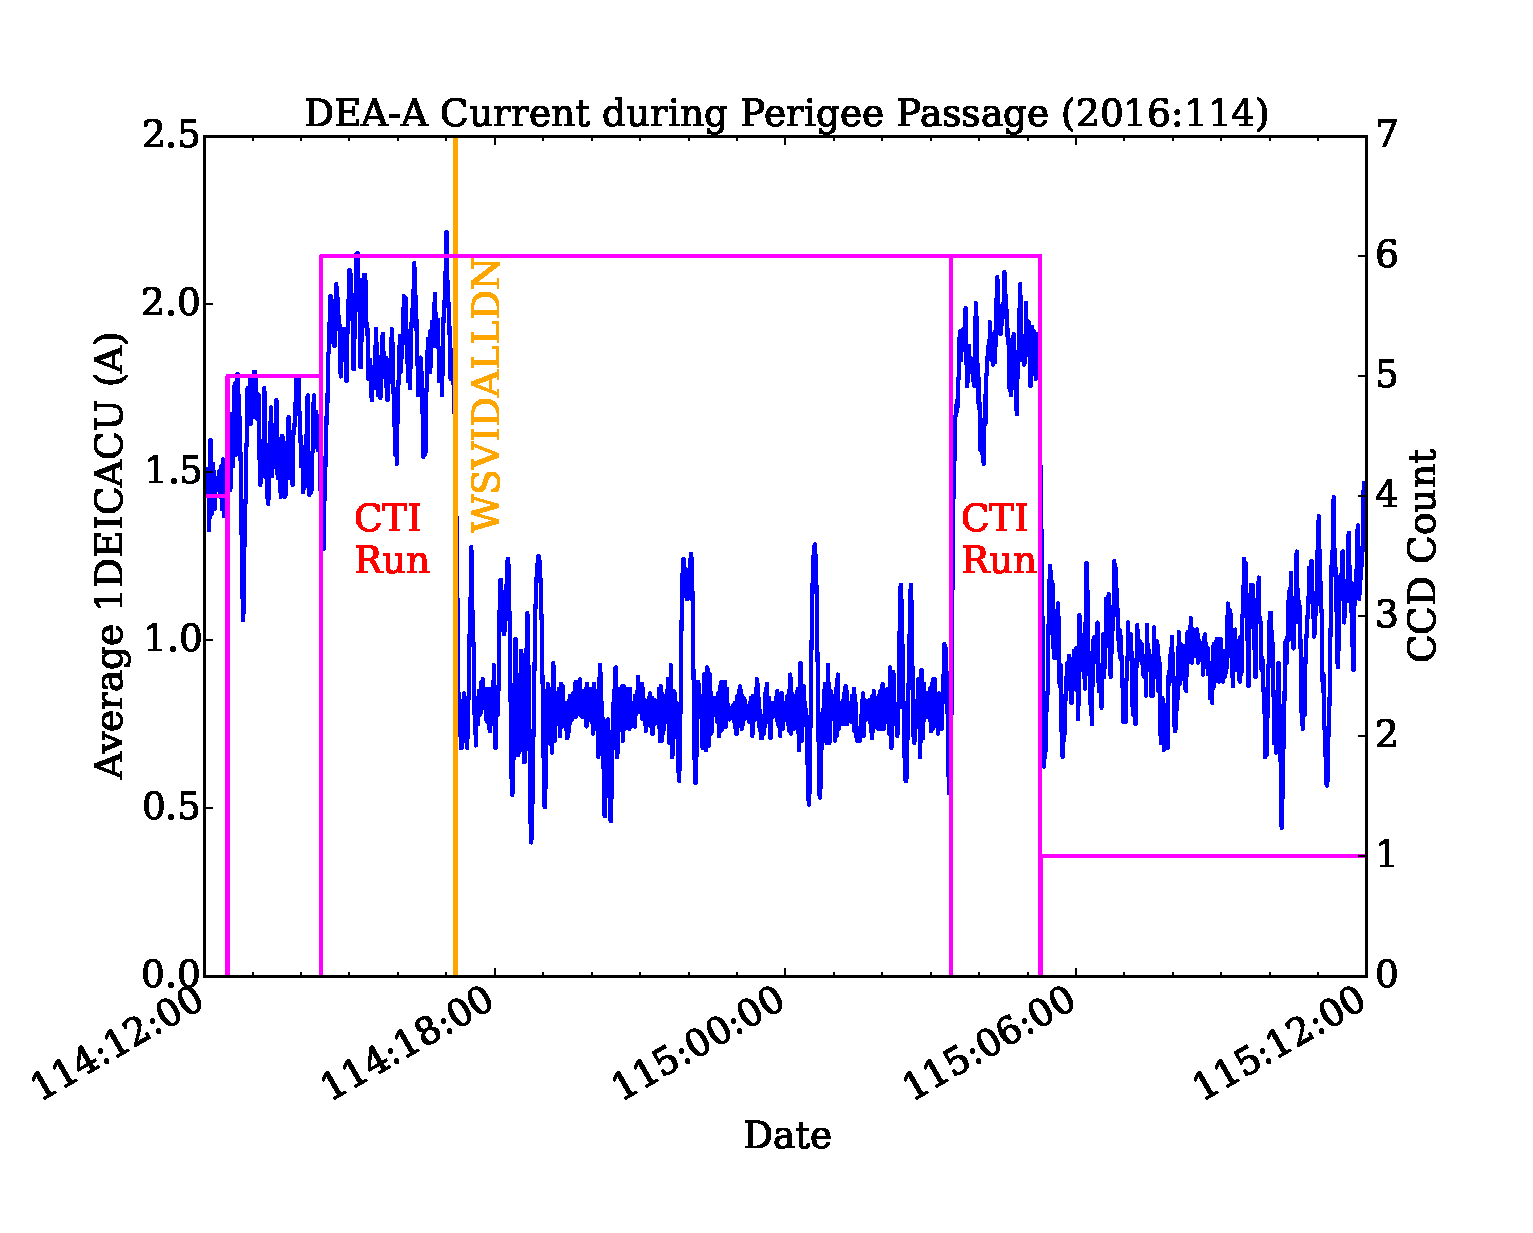
\includegraphics[width=1.2\textwidth]{deaa_on_fig1.eps}
\caption{Ten-sample running average behavior of 1DEICACU during a perigee passage. All video boards
are powered off after the issuing of the WSVIDALLDN command, which is marked by
the orange line in the plot.}
\end{center}
\end{figure}
\end{landscape}

\begin{landscape}
\begin{figure}
\begin{center}
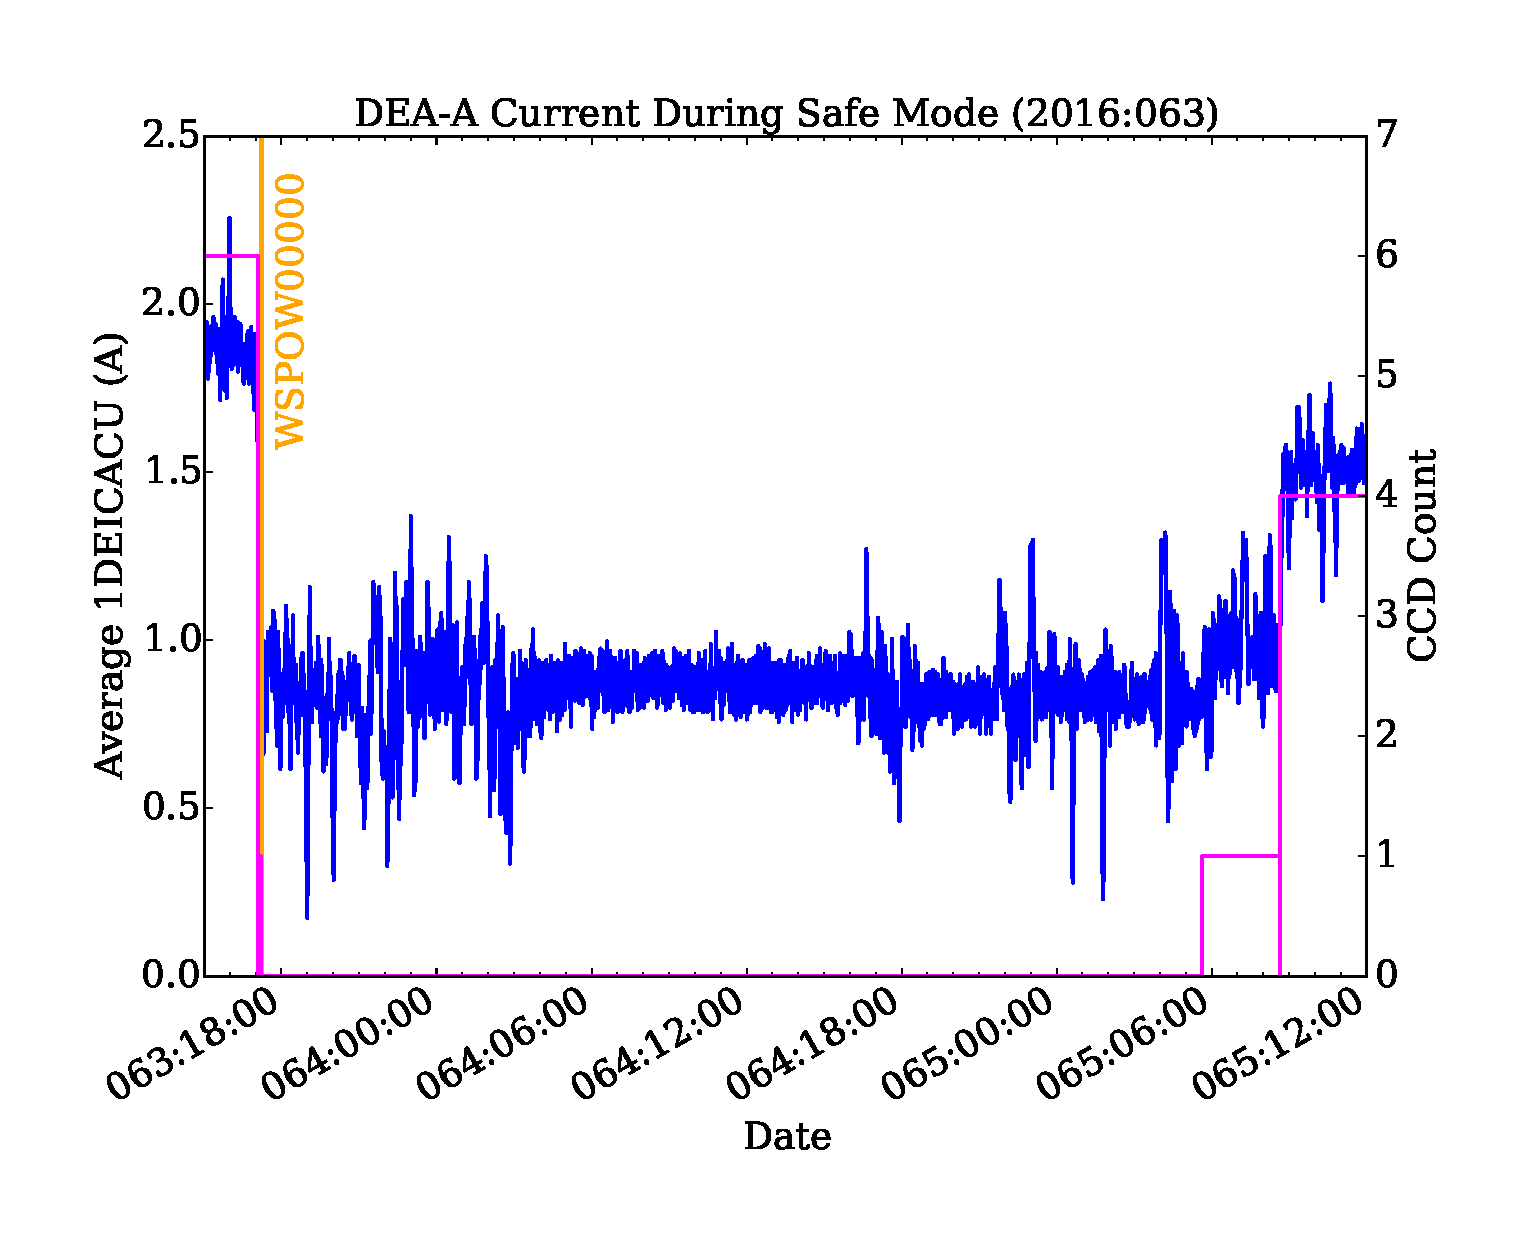
\includegraphics[width=1.2\textwidth]{deaa_on_fig2.eps}
\caption{Ten-sample running average behavior of 1DEICACU during a safe mode. All video boards
are powered off after the issuing of the WSPOW00000 command, which is marked by
the orange line in the plot.}
\end{center}
\end{figure}
\end{landscape}

\newcommand{\tablecaptiontext}{TURN ON DEA A}
\documentclass[11pt]{article}

\usepackage{lscape,color}
\usepackage{graphicx}
\usepackage[normalem]{ulem}

\topmargin -0.75truein
\oddsidemargin -0.4truein
\textheight 9.25truein
\textwidth 6.7truein
\hbadness=10001
\hfuzz=200pt


\begin{document}
%\input dspace12.tex
%\input pstricks.tex
%\input psfig
\newcommand{\be}{\begin{enumerate}}
\newcommand{\ee}{\end{enumerate}}
\newcommand{\bc}{\begin{center}}
\newcommand{\ec}{\end{center}}
\newcommand{\bi}{\begin{itemize}}
\newcommand{\ei}{\end{itemize}}
\newcommand{\bd}{\begin{description}}
\newcommand{\ed}{\end{description}}
\newcommand{\bt}{\begin{tabbing}}
\newcommand{\et}{\end{tabbing}}
\newcommand{\eg}{{\it e.g.~}}
\newcommand{\ie}{{\it i.e.~}}
\newcommand{\ul}{\underline}
\newcommand{\axaf}{{\em AXAF}}

\def\la{\hbox{\rlap{$<$}\lower0.5ex\hbox{$\sim$}\ }}


\large
%\vspace*{-0.5in}
\centerline {\bf 4.5\_V2.6 TURN ON DEA A}
\vspace{0.25in}

\normalsize
\noindent{\it Last Revised: July 11, 2017}\\
\noindent{\bf Filename: deaa\_on} \\


\noindent {\bf BRIEF FUNCTIONAL DESCRIPTION:} \\
\normalsize
This is an ``atomic'' procedure which simply powers up the DEA side A.
It should be safe to execute under any condition except a spacecraft 
power or thermal emergency.

\vspace{0.25in}
\noindent The sequence of actions for this procedure will be:
\be
\item Verify that DEA B is powered off and disabled (see Constraints/Cautions, below)
\vspace{-0.10in}
\item Verify that DEA A is receiving power from the spacecraft
\vspace{-0.10in}
\item Enable and turn on DEA power supply side A
\vspace{-0.10in}
\item Verify that DEA B is still off
\ee

\vspace{0.15in}
\normalsize
\noindent {\bf ASSUMED INSTRUMENT STATE:}
\normalsize
\be
\item Assumes that the PSMC has power from the spacecraft.
\vspace{-0.10in}
\item Assumes that DEA B is off.
\ee
\vspace{0.1in}
\normalsize
\noindent {\bf SPECIAL INITIAL CONDITIONS:} \\
\normalsize
%The environment must be clean enough to allow opening of the valve. \\
%Assumes that \axaf\/ ISIM RCTU is powered on and in telemetry format 6. \\

%\vspace{0.25in}
\normalsize
\noindent {\bf OPERATIONAL CONSTRAINTS/CAUTIONS:} \\
\normalsize

In normal operations, only one side of the DEA should be powered on
(a) to prevent conflict for control of the focal plane temperature controller,
(b) to avoid excess current draw from the spacecraft, and (c) to avoid over-heating
within the PSMC.

The DEA power status is normally indicated by the values of the 1DEPSA and
1DEPSB flags, which should not both be 1 simultaneously.
However, if neither side of the DPA is receiving power
({\it i.e.}, if 1DPP0AVO and 1DPP0BVO are simultaneously reading $0.0 \pm 0.5$ V),
the DEA flag values will be unreliable and the DEA voltage
channels (1DEP[0123][AB]VO) should instead be used to determine which
sides of the DEA are powered).

Before sending the command to power on DEA A, the DEA Input Voltage A 1DE28AVO should
be checked to make sure that DEA A is receiving power from the spacecraft.

The DEA input current monitors (1DEIC[AB]CU) are noisy.
To give an indication of what variation may be expected, figures 1 and 2
show the behavior of the A-side DEA current with a ten-sample running
average for two situations in which all video boards were powered down. Note that
when either side of the DEA is unpowered, the corresponding current monitor, 
1DEICACU for side A, or 1DEICBCU for side B, will be unreliable. They will read
16--18~A when unpowered, as of Telemetry Database (TDB) v14. This is expected and
not a problem.

If the DEA powers off unexpectedly during a bakeout, the FP bakeout 
heater will lose power and this heater will NOT be re-enabled when the DEA side A 
power is restored. Additional SW commands are necessary to activate the FP bakeout 
heater. The DH bakeout heater is unaffected by a power loss to the DEA and will 
therefore still be executing a bakeout if power is lost to the DEA.

After successful execution, {\em the FP temperature control will be unregulated,
and DEA interface A/D will be in low-resolution mode.}\\

\vspace{0.15in}
\normalsize
\noindent {\bf REFERENCES:} \\
\normalsize

\normalsize
\noindent {\bf CHANGE HISTORY:} \\
\normalsize

{\bf V1.2}
\begin{itemize}
\item changed filenames from ``turnon\_deaa'' to
``deaa\_on''
\item added text to explain the confusion with the logical verifiers
\end{itemize}

{\bf V1.3}
\begin{itemize}
\item changed HW TLM verifier in step 1.2 to ``1DEN1AVO'' from
``DEN1AVO''
\item changed criticality of +24~V to 1
\item changed TLM FMT to 1,2,4or6
\item added step 1.3 to verify that DEA B is still off
\item added comments to warn that the FP temp will be set to 0~K after the DEA A is powered
\end{itemize}

{\bf V2.0}
\begin{itemize}
\item ACIS Team signed-off version
\item changed HW TLM verifier in step 1.3 to ``1DEN1BVO''
\item edited ``Operational Constraints \& Cautions''
\end{itemize}

{\bf V2.1}
\begin{itemize}
\item Update expected 1DE28AVO range
\item Changed formatting of ``Tlm Fmt'' in table
\item Changed time column from units of seconds to minutes in table
\item Changed text in table column ``Description''
\item Updated expected voltage errors in Step 1.3
\end{itemize}

{\bf V2.2}
\begin{itemize}
\item Update expected 1DEICACU range
\item Add plots showing the behavior of 1DEICACU
\end{itemize}

{\bf V2.3}
\begin{itemize}
\item Added a step to verify DEA-B is off at the beginning of the procedure
\item Moved the text regarding power status issues and expected current behavior from the Functional Description to the Operational Constraints/Cautions section. Also updated the expected FP temperature control.
\end{itemize}

{\bf V2.4}
\begin{itemize}
\item Fixed incorrect 1DEN0AVO and 1DEN1AVO voltages in table
\end{itemize}

{\bf V2.5}
\begin{itemize}
\item Removed input current check for DEA B; added warning to text.
\end{itemize}

{\bf V2.6}
\begin{itemize}
\item Added check of input voltage for DEA A before sending the turn-on command
\item Adjusted values of ``Crit'' column in table. 
\item Note that a bakeout will be interrupted if the DEA powers off, provide details
\end{itemize}

\begin{landscape}
\begin{figure}
\begin{center}
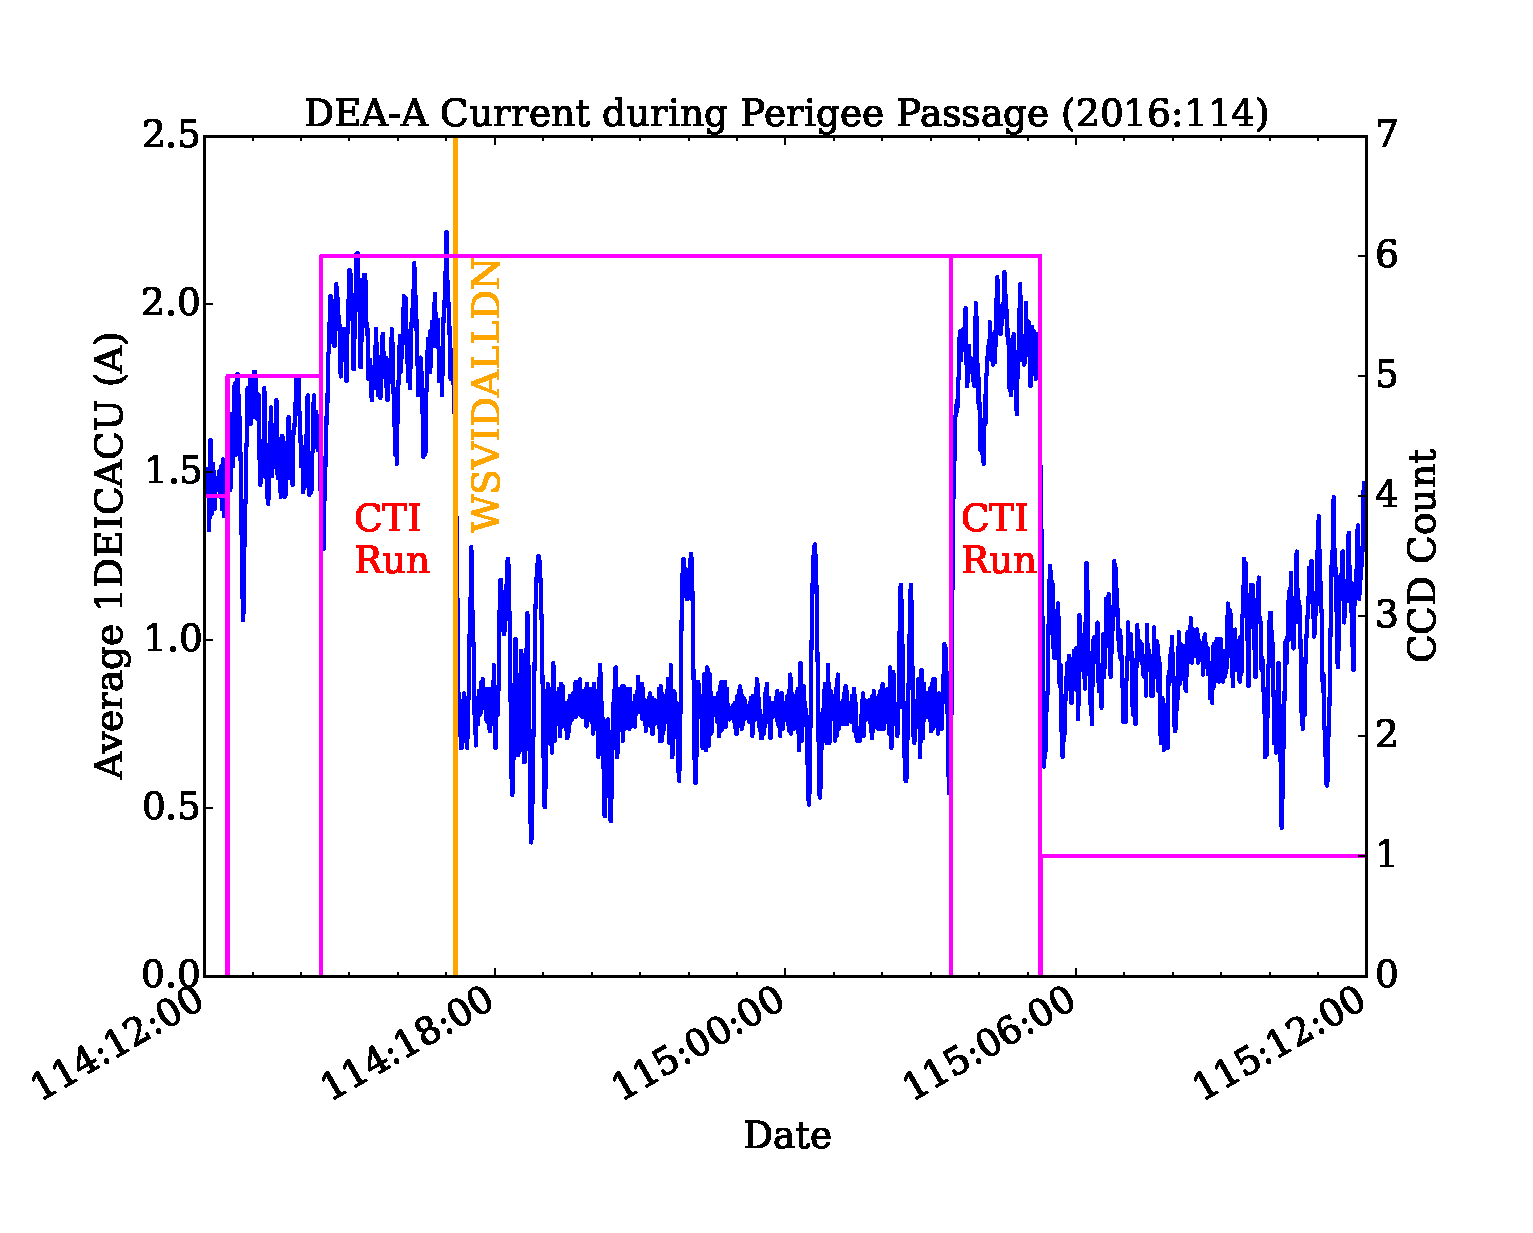
\includegraphics[width=1.2\textwidth]{deaa_on_fig1.eps}
\caption{Ten-sample running average behavior of 1DEICACU during a perigee passage. All video boards
are powered off after the issuing of the WSVIDALLDN command, which is marked by
the orange line in the plot.}
\end{center}
\end{figure}
\end{landscape}

\begin{landscape}
\begin{figure}
\begin{center}
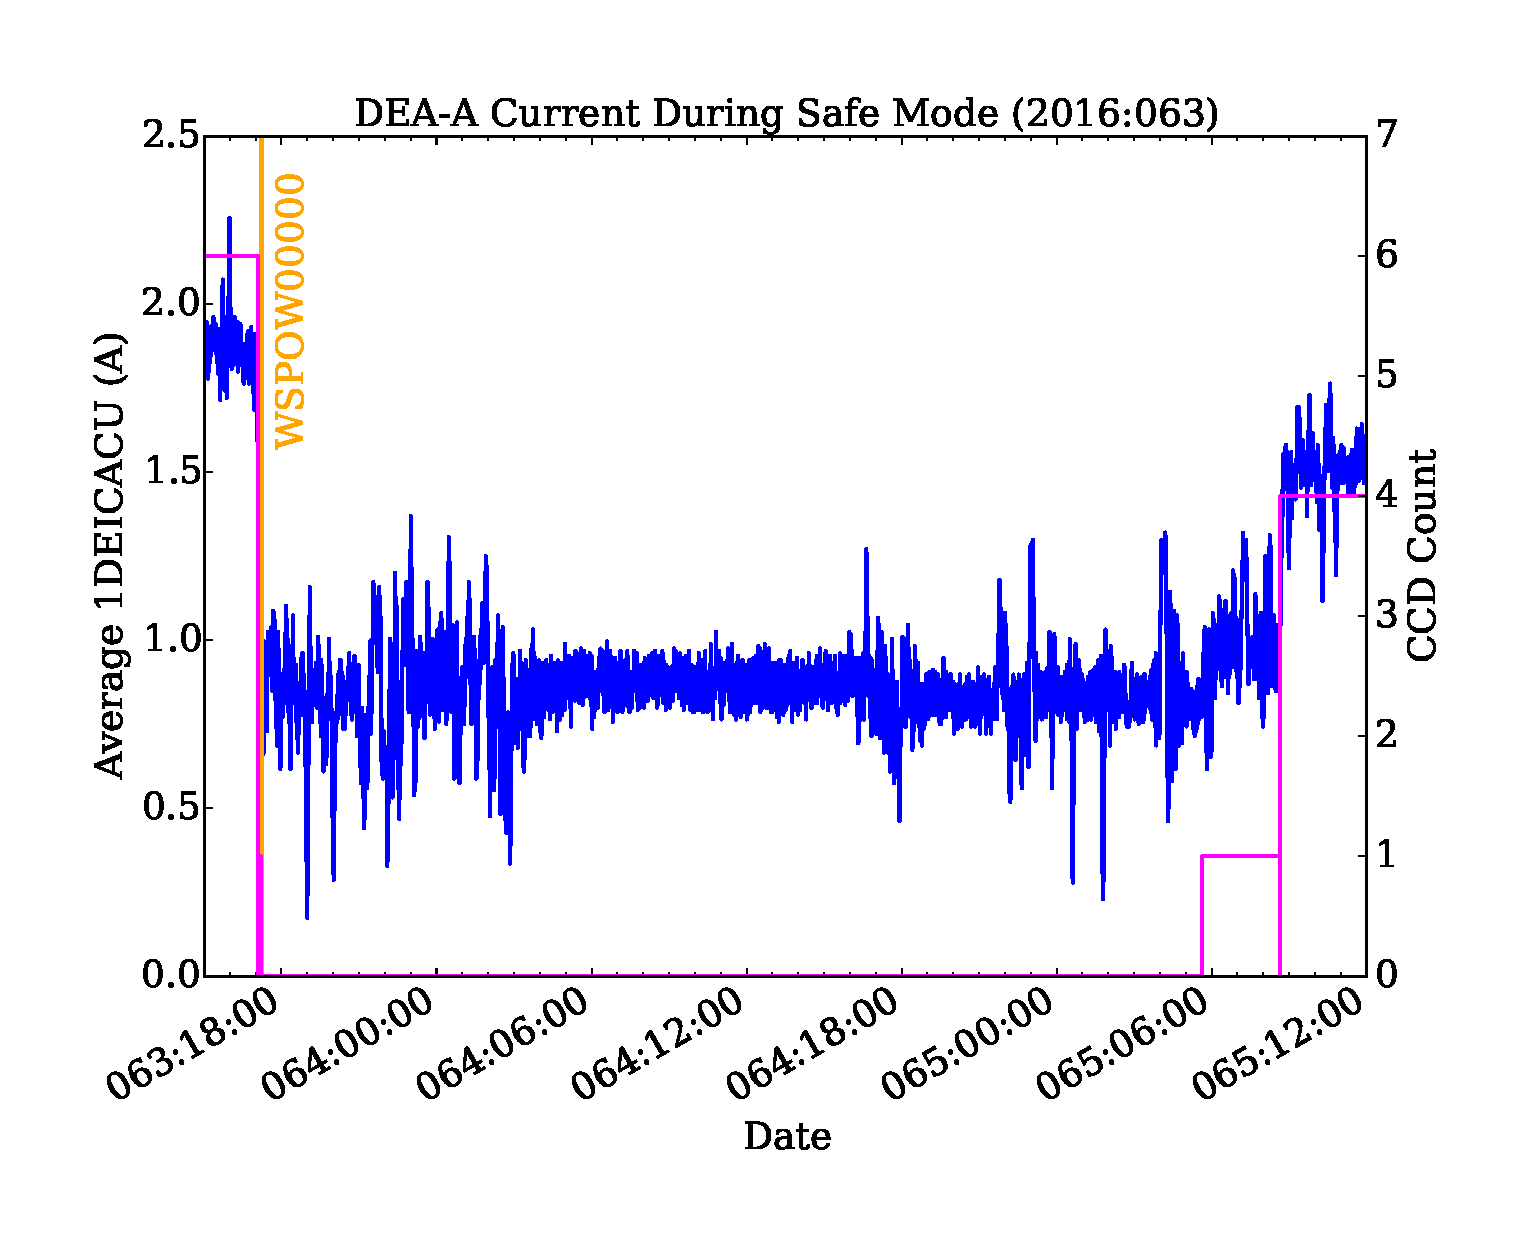
\includegraphics[width=1.2\textwidth]{deaa_on_fig2.eps}
\caption{Ten-sample running average behavior of 1DEICACU during a safe mode. All video boards
are powered off after the issuing of the WSPOW00000 command, which is marked by
the orange line in the plot.}
\end{center}
\end{figure}
\end{landscape}

\newcommand{\tablecaptiontext}{TURN ON DEA A}
\input{deaa_on.tab}

\end{document}


\end{document}


\end{document}


\end{document}
